\documentclass{template/openetcs_article}
% Use the option "nocc" if the document is not licensed under Creative Commons
%\documentclass[nocc]{template/openetcs_article}
\usepackage{lipsum,url}
\usepackage{supertabular}
\usepackage{multirow}
\usepackage{color, colortbl}
\definecolor{gray}{rgb}{0.8,0.8,0.8}
\usepackage[modulo]{lineno}
\graphicspath{{./template/}{.}{./images/}}
\begin{document}
\frontmatter
\project{openETCS}

%Please do not change anything above this line
%============================



% The document metadata is defined below

%assign a report number here
\reportnum{OETCS/WP1/D02}

%define your workpackage here
\wp{Work-Package 7: ``Toolchain''}

%set a title here
\title{Requirements Modeling for SSRS Activities with ProR}

%set a subtitle here
\subtitle{Results of ProR/SSRS Workshop in Braunschweig}

%set the date of the report here
\date{October 8, 2013}

%define a list of authors and their affiliation here

\author{Michael Jastram}

\affiliation{Formal Mind GmbH}

% define the coverart
\coverart[width=300pt]{img/pror-splash.png}

%define the type of report
\reporttype{Position Paper}


\begin{abstract}
During the Braunschweig workshop on October 8th, we had a small work session to start modeling the SSRS requirements in ProR.  Participants were:

\begin{itemize}
\item Uwe Steinke
\item David Mentre
\item Jan Welvaarts
\item Michael Jastram
\end{itemize}

The objective was to start a trial migration of the refined requirements created by Jan, in the context of the SSRS activities.

\end{abstract}

%=============================
\maketitle

%Modification history
%if you do not need a modification history table for your document simply comment out the eight lines below
%=============================
\section*{Modification History}
\tablefirsthead{
\hline 
\rowcolor{gray} 
Version & Section & Modification / Description & Author \\\hline}
\begin{supertabular}{| m{1.2cm} | m{1.2cm} | m{6.6cm} | m{4cm} |}
 0.1 & all & Michael Jastram& \\\hline
\end{supertabular}


\tableofcontents
\listoffiguresandtables
\newpage
%=============================

%Uncomment the next line if you need line numbers for tracebility when the document is in review
%\linenumbers
%=============================


% The actual document starts below this line
%=============================

%Start here

\section{SRS Data Model}

Jan Welvaarts already spent some time creating a document using OpenOffice, representing a subset of the SSRS.  We captured this on a whiteboard (upper part of Figure~\ref{fig:whiteboard}.  A first attempt to capture this with the data structures available by ProR is shown in the lower part.  That part has been cleaned up and is shown in Figure~\ref{fig:ssrs_elements}.

\begin{figure}
	\begin{center}
	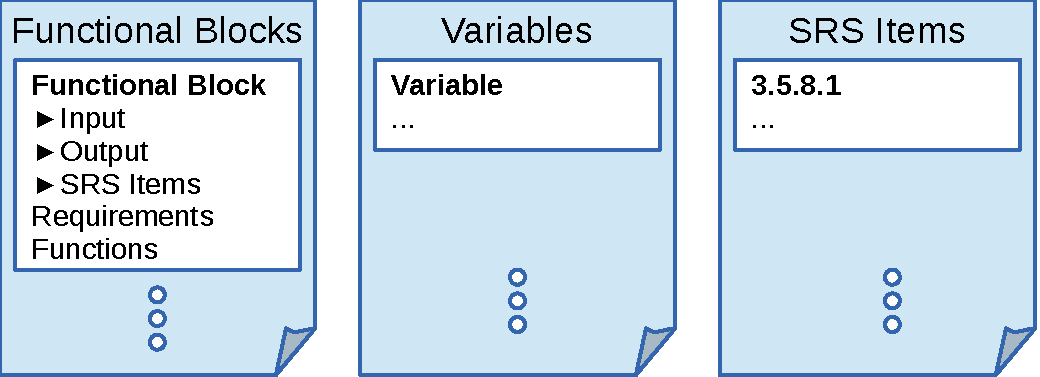
\includegraphics[width=0.6\textwidth]{img/relationships.pdf}
	\end{center}
	\caption{The major elements of the SSRS.}
	\label{fig:ssrs_elements}
\end{figure}

In the following, we will describe the elements from these figures.

\begin{description}

\item[Functional Block.] A \emph{Functional Block} contains a set of \emph{Functions}.  Each \emph{Function} can be referenced from multiple \emph{Functional Blocks}.  It contains references to \emph{Imputs}, \emph{Outputs} (which are \emph{Variables}) and \emph{SRS Items}.  It also contains an arbitrary number of \emph{Requirements}.

\item[Function.] An element of a \emph{Functional Block} with \emph{Imputs} and \emph{Outputs}.

\item[Variable.] \emph{Variables} are explicitly listed in the SRS (e.g. those extracted by the BitWalker Scripts).  They can also appear implicitly in the requirements text of the SRS.  The \emph{Variables} referenced from \emph{Functional Blocks} are typically compound structures consisting of multiple \emph{Variables}.

\item[Input.] A \emph{Variable} that is used as an input for a \emph{Function} or \emph{Function Block}.

\item[Output.] A \emph{Variable} that is used as an input for a \emph{Function} or \emph{Function Block}.

\item[SRS Item].  The SRS consists of \emph{SRS Items}.  Most of the time, it is a paragraph, which has an ID (e.g. 3.5.7.5.3).  Due to the heterogeneous nature of the SRS document, it can sometimes be something else ( a table, a sentence, a group of items, etc.).

\end{description}

\section{ProR Data Model}

We prototypically built data structures in ProR, which can be used to represent the previously described data model.  In the following, we will describe this data structure.  It is also stored on gitHub at

\url{https://github.com/openETCS/SSRS/trunk/Requirements_Modeling}

In ProR, we organized the model into three top level \emph{Specifications} (document-like structure that each contain a tree of elements): \emph{Functional Blocks}, \emph{Variables} and \emph{SRS Items}.

\subsection{SRS Items}

In the \emph{SRS Items}, one \emph{SpecObject} per \emph{SRS Item} is created.  For now, this will just be an element with ID, and optionally some explanatory text.  Later, this could be converted into a proxy element to provide an integrated traceability into the SRS.  But this requires additional work.  The figure below shows this, for two (dummy) entries:

\begin{center}
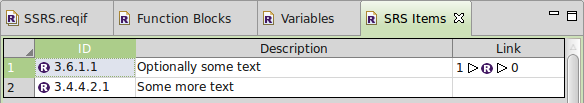
\includegraphics[width=0.8\textwidth]{img/srs-items.png}
\end{center}

The \emph{Link} columns indicates thast the item 3.6.1.1 has one incoming link, meaning that there is one \emph{Function Block} referencing it.

\subsection{Variables}

At least for the time being, \emph{Variables} will be handled like \emph{SRS Items}.  But note that they are usually compound structures, which is handled through nesting, as shown below.  This kind of nesting would be possible for the \emph{SRS Items} as well.

\begin{center}
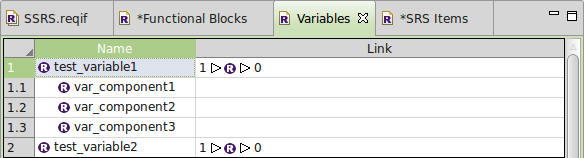
\includegraphics[width=0.8\textwidth]{img/variables.png}
\end{center}

Eventually, the work done by Siemens with the BitWalker tool could be used here by directly referencing the variables from the generated XML document.

\subsection{Functional Blocks}

The \emph{Functional Blocks} essentially pull the other information together and augment it.  This is shown below.

\begin{center}
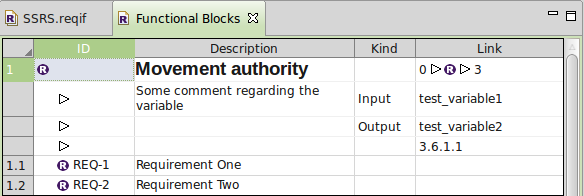
\includegraphics[width=0.8\textwidth]{img/functional-blocks.png}
\end{center}

The name of the \emph{Functional Block} is shown in a bigger font (realized with the ProR Headline plugin).  This element has three outgoing traces: one \emph{Input}, one \emph{Output} and one \emph{SRS Item}.  These traces have attributes, and the links to the \emph{Variables} contain an attribute called \emph{Kind}, which classifies it (this is an enumeration attribute).

Realized as child elements (therefore indented), two additional \emph{Requirements} have been added.  The human-readable IDs have been generated by another ProR plugin.

Missing from the picture are the actual \emph{Functions}, which will be discussed in the next section.

\subsection{Functions}

We didn't decide yet on how to model the \emph{Functions}.  From a usability point of view, simly adding them to the \emph{Function Blocks} would be a good solution (indenting them by taking advantage of the tree structure).  However, as \emph{Functions} can be referenced by multiple \emph{Functional Blocks}, a link may be better (but less readable).  The readability issue could be addressed by generating reports that inline the \emph{Functions}.  ProR also allows referencing elements.  Thus, multiple \emph{Function Blocks} could simply point to the same \emph{SpecObjects} that represent the \emph{Functions}.  This can still create inconsistencies.  For instance, if a \emph{Function} is extended by a \emph{SpecObject} (to add some additional information, for instance), a reference to that SpecObject would have to be added to all places where this \emph{Function} is referenced.

\subsection{A Note about Text Formatting}

So far, only plain text has been used.  We suggest the usage of plain text for two reasons: First, using plain text will make model integration later on much easier, as color highlighting, parsing, etc. are much easier on plain text.  Second, while ProR has rich text support, it is not very good and has limitations on some platforms (e.g. on Mac).

The team generally considered plain text sufficient, except that logical expressions are much more readable when formatted.

\section{SysML Integration}

So far, SysML integration has not been discussed at all, but should be eventually be covered in this document as well.

Integrating ProR and Papyrus will be relatively easy, and will be made available by Michael, as a contribution to this project.  The integration will work as follows: ProR will be installed into Papyurus (or the other way around).  The Papyurs Model Browser must be opened, which allows access to all SysML elements.  Linking will be performed by dragging from the Model Browser onto the corresponding \emph{SpecObject}.

The first version of the integration plugin will show a textual representation of the corresponding SysML element in ProR (e.g. the Block Name or Port Name).

\section{Backlog}

In this section, we collect tasks that need to be done in order to make work with ProR practical.  These are listed here in no particular order.  Eventually, they should make their way into the WP7 backlog, to be implemented:

\begin{description}

\item[Reporting.] While rudimentary reporting is available (via the print functionality, which generates HTML), we almost certainly will need tailored reporting for acceptance.

\item[SRS Traceability.]  The traceability to the SRS suggested here is just a crutch.  We either need a traceability into the Word documents, or we need to import the SRS into ProR.  Both approaches have their respective advantages and disadvantages.

\item[SysML/Papyrus Traceability.]  This has been discussed earlier.

\item{Formatting Logical Expressions.} As mentioned earlier, logical expressions would benefit from using formatted text.  This either requires improving rich text support, or the creation of a dedicated representation for logical expressions (e.g. by using a DSL).

\end{description}

\section{Appendix: Whiteboard}

\begin{figure}[h!t]
	\begin{center}
	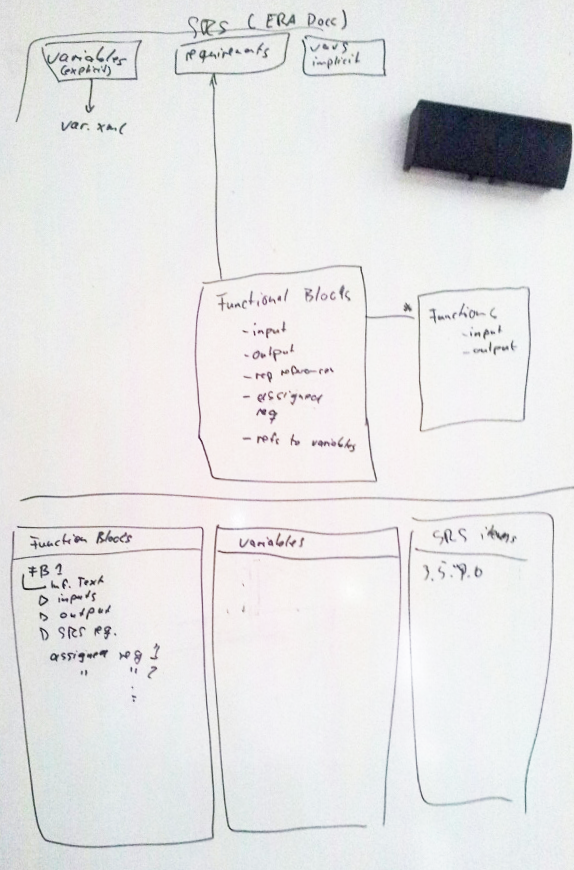
\includegraphics[width=0.8\textwidth]{img/whiteboard.png}
	\end{center}
	\caption{The whiteboard content that outlines the ProR data model.}
	\label{fig:whiteboard}
\end{figure}


% \bibliographystyle{unsrt}
% \bibliography{erdc}


%===================================================
%Do NOT change anything below this line

\end{document}
